
\aaa{Vector Spaces}
Geometrically, vector spaces are \x{infinitely extended},\x{flat} spaces \x{with a selected origin}. 
\vfill
\[columns]{\co{35}
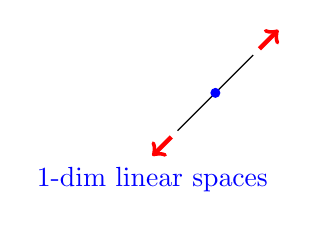
\begin{tikzpicture}[scale =0.8]
    \draw (0,0)--(1.2,1.2);
    \draw[->,red,ultra thick](-.1,-.1)--(-.4,-.4) node[below,blue]{1-dim linear spaces};
    \draw[->,red,ultra thick](1.3,1.3)--(1.6,1.6);
    \draw[fill,blue] (0.6,0.6) circle[radius=0.07];
\end{tikzpicture}
\co {35}
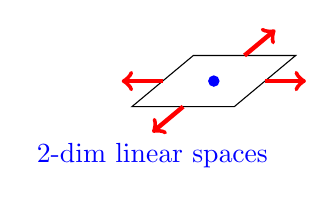
\begin{tikzpicture}[scale = 1.3]
    \draw (1,0)--(1.6,0.5)--(0.6,0.5)--(0,0)--(1,0);
    \draw[->,red,ultra thick](0.5,0)--(0.2,-0.25) node[below,blue]{2-dim linear spaces};
    \draw[->,red,ultra thick](1.1,0.5)--(1.4,0.75);
    \draw[->,red,ultra thick](0.3,0.25)--(-0.1,0.25);
    \draw[->,red,ultra thick](1.3,0.25)--(1.7,0.25);
    \draw[fill,blue] (0.8,0.25) circle[radius=0.05];
\end{tikzpicture}
\co 3
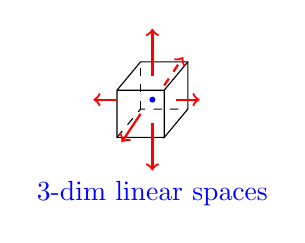
\begin{tikzpicture}[scale =0.6]
    \draw (1,0)--(0,0)--(0,1)--(1,1)--(1,0)--(1.5,0.6)--(1.5,1.6)--(0.5,1.6)--(0,1);
    \draw (1,1)--(1.5,1.6);
    \draw[dashed] (0,0)--(0.5,0.6)--(1.5,0.6);
    \draw[dashed] (0.5,0.6)--(0.5,1.6);
    \draw[->,red,thick](1.25,0.8)--(1.75,0.8);
    \draw[->,red,thick](0,0.8)--(-0.5,0.8);
    \draw[->,red,thick](0.5,0.5)--(.1,-.1);
    \draw[dashed,->,red,thick](1,1.1)--(1.4,1.7);
    \draw[->,red,thick](0.75,0.3)--(0.75,-0.7) node[below,blue]{3-dim linear spaces};
    \draw[->,red,thick](0.75,1.3)--(.75,2.3);
    \draw[fill,blue] (0.75,0.8) circle[radius=0.05];
    
\end{tikzpicture}

Here the red arrow means the actual object is extending, not only what you saw in the picture.
}
\a\aa
\raisebox{1.6cm}{
\begin{defi}
	An \textbf{$ℝ$-vector space}  is a set $V$, equipped with an operator "+" and scalar multiplication from $ℝ$ satisfying 
    \begin{enumerate}
   	    \item [1.0)] For any $\vec v,\vec w\in V$, $\vec v+\vec w$ is an element in $V$;
	    %\item [1.1)] \x{(not necessary)} For any $\vec v,\vec w\in V$, $\vec v+\vec w=\vec w+\vec v$;
	    \item [1.2)] For any $\vec v,\vec w,\vec u\in V$, $(\vec u+\vec v)+\vec w=\vec u+(\vec v+\vec w)$;
	    \item [1.3)] There exists $\vec0\in V$ such that for any $\vec v\in V$, $\vec0+\vec v=\vec v$;
	    \item [1.4)] For any $\vec v\in V$, There is $-\vec v\in V$ such that $\vec v+(-\vec v)=0$;
    \item [2.0)] For any $\vec v\in V$, $\lambda \in ℝ$, $\vec v\cdot \lambda$ defines an element in $V$;
    \item [2.1)] For any $\vec v\in V$, $\vec v\cdot 1=\vec v$;
    \item [2.2)] For any $\vec v\in V$, $\lambda,\mu \in ℝ$,$\vec v\cdot (\lambda\mu)=(\vec v\cdot\lambda)\cdot\mu$;
    \item [2.3)] For any $\vec v\in V$, $\lambda,\mu\in ℝ$,$\vec v\cdot(\lambda+\mu)=\vec v\cdot\lambda+\vec v\cdot\mu$;
    \item [2.4)] For any $\vec v,\vec w\in V$, $\lambda\in ℝ$,$(\vec v+\vec w)\cdot\lambda=\vec v\cdot\lambda+\vec w\cdot\lambda$.
    \end{enumerate}
\end{defi}
}
%\a{Comments}
%While seeing this definition, it is important to know that
%\[itemize]{
%\item A vector can be anything other than just an arrow, as long as there are predescribed operators $+$ and $\cdot$ satisfying these axioms.
%\item When describing a vector space, we must clearify it as a set $V$, and define what the addition and scaling means for it. We can not claim a vector space before confirming that our predefined operators satiesfies these axioms.
%\item Note that by $\QQ$-vector space we mean that one can only scale a vector by scalars in $\QQ$, whereas by $\RR$-vector spaces we mean that one can use scalrs in $\RR$. It is important to claim that which field $F$ the vector space is over to avoid confusions. From now, you can just assume $F=\RR$.
%\item The axiom of commutativity is not necessary since it can be deduced from other axioms.
%}
%
\a{Examples of vector spaces--Geometry}
The flat, infinitely extended lines or planes with selected origins are the most common vector spaces, where each point is identified with the end point of each vector starting from the origin. The addition is defined by the parallelogram law and the scalar multiplication is defined by the usual scaling.  

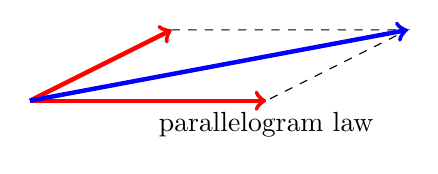
\begin{tikzpicture}[scale=3]
\draw[->,ultra thick,red](0,0)--(0.6,0.3);
\draw[->,ultra thick,red](0,0)--(1,0) node[below,black]{parallelogram law};
\draw[dashed](0.6,0.3)--(1.6,0.3)--(1,0);
\draw[->,ultra thick,blue](0,0)--(1.6,0.3);
\end{tikzpicture}
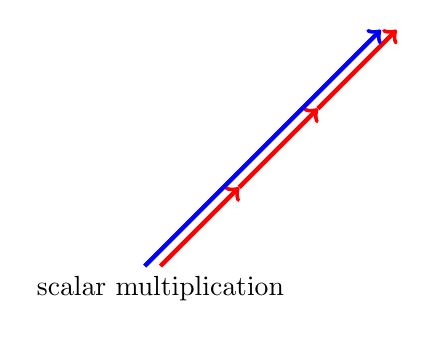
\begin{tikzpicture}
\draw[->,ultra thick,red](0,0)--(1,1);
\draw[->,ultra thick,red](1,1)--(2,2);
\draw[->,ultra thick,red](2,2)--(3,3);
\draw[->,ultra thick,blue](-0.2,0)--(2.8,3);
\node[below] (0,0){scalar multiplication};
\end{tikzpicture}

\bb{Question: What is zero vector in this space?}

\a{Abstraction}
Not all vector spaces can be described in such a geometric and intuitive way, but this is the only way for data visualization.
\vfill
Shinchan has a coffee shop. He wants to treat the recipe of each dish as a vector intuitively, what should he do?
\a\aa
\no: Are they vectors also? \fbox{\leaf\bean\bean},\; \fbox{\leaf\bean},\; \fbox{\leaf\leaf\bean}.
~\\

\buxie: There are no arrows like \[tikzpicture]{\draw[red,thick,->](0,0)--(1,0);} .
~\\
\no: But I'd still say --- vectors!
~\\
\buxie: If you like.
~\\
\sinister: Actually, you can, as long as you define the addition and the scalar multiplication properly! Everything can be a vector.~\\
\tear
\a\aa

\homework: I don't believe, how? Show me arrows!

\boss: I can do it! Let me show you!

\a{Vector space: Package of Materials}
Abstract vector spaces can be visualized by linear combinations.

Here is the way how Shinchan represent each of the vegetable package intuitively in the space. How?
\[columns]{
	\co 7
\[z]{
\org
%\xaxis{-1}5
%\yaxis{-1}5
\grid{-3}{-3}33
%\wangge
\draw (1,0) node {\leaf} (0,1) node {\bean};
\nnw A12
\nnw B11
\nnw C21
	}
\co3
A= \fbox{\leaf\bean\bean}~\\
\vspace{1cm}

B=\fbox{\leaf\bean}~\\

\vspace{1cm}
C=\fbox{\leaf\leaf\bean}
}
1
\a\aa
As long as your definition of vector spaces satiesfy these axioms, it is always valid to substitute your data by some arrows. For example, position $C$ is obtained by replacing \leaf by $\rightarrow$, and \bean by $\uparrow$.
\[columns]{
	\co 7
\[z]{
\org
\grid{-3}{-3}33
\draw (1,0) node {\leaf} (0,1) node {\bean};
\nnw C21
\draw[->,ultra thick,green!70!black] (0,0)--(1,0) ;
\draw[->,ultra thick,green!70!black] (1,0)--(2,0);
\draw[->,ultra thick,red!70!black] (2,0)--(2,1);
	}
\co3
C=\fbox{\leaf\leaf\bean}

\vspace{1cm}

\leaf:$\rightarrow\qquad$\bean:$\uparrow$

\vspace{1cm}

C:\fbox{$\rightarrow$ $\rightarrow$ $\uparrow$}

}

\a{Abstract vector space v.s. intuitive vector space }
You can always visualize a vector space by an intuitive vector space by this method. But in general, \x{they are not the same}. It is simply because you can only visualize it after a choice of replacement by arrows, but the element in a vector space itself should not be always arrows --- it could be vegetables, human, airplane or whatever as long as you can define addition and scalar multiplication that satisfy axioms.
%\a\aa
%
%In this space, each point is a certain linear combination of materials. To specify a package, we need to know how much is each materials in this package.%, the desctiption of points in this space is \enuv.
%\vfill
%
%In these slides, we call this space where each point indicates a linear combination, the \x{space of linear combination}.(or space of combination for short)
%
%\bb{Question: What kind of package(or linear combination) is representing the zero vector in this space?}
%4
\a{Examples of vector spaces--$n\times 1$ matrices}
The set of all $n\times 1$ matrices over $ℝ$ is denoted by $ℝ^n$, which is a vector space by the following structure: The sum of two matrices is just the normal sums. the scalar multiplication is naturally obtained by scaling each entries. For example.\par
$$
\m{2},{3},{1}.+\m{1},{5},{0}.=\m{3},{8},{1}.\text{vector addition}
$$
$$
\m{5},{1},{2}.5=\m{25},{5},{10}.\text{scalar multiplication},
$$
\bb{Question: What is zero vector in this space?}

\a{Examples of vector spaces--Polynomials}
Let $\lPP xabc$ be the set of polynomials of degree at most 2 with real number coefficients. It is a vector space over $\RR$ in the following sense: The addition structure is the sum of two polynomials, the scalar multiplication is multiplying a constant. 
$$
(x^2+1)+x=x^2+x+1\text{   vector addition}
$$
$$
3(x^2+1)=3x^2+3\text{   scalar multiplication}
$$
\vfill
\bb{Question: What is zero vector in this space?}

%\a{Value Table of polynomials}
%The linear space $\lPP xabc$ looks different from what you learned before. How do we understand it as vectors? If you like the idea of list of numbers, we can also transform it into a list of number, by the following \bb{Value Table}. Different choice of evaluation gives you different value table
%\vfill
%\[columns]{\co 4
%\t{F}1{x}{$x^2$},{F(0)}100,{F(1)}111,{F(2)}124.
%\co 4
%\t{F}1{x}{$x^2$},{F(0)}100,{F'(0)}010,{F''(0)}00{2}.
%}
%\vfill
%This suggests we can think functions as a list of number if you tell me how to create the list. By $F(0),F(1),F(2)$ or $F(0),F'(0),F''(0)$ or others. In the future you will see both of the two table determines elements in $P_2$ completely.
\a{Example of vector spces -- Rational functions}
A rational function is a quotient of two polynomials. For example, the set 
$$
%V=\frac{P^2_x}{(x+1)(x+2)(x+3)}:=
\left\{f: f(x)=\frac{x^2a+xb+c}{(x+1)(x+2)(x+3)} \text{ for some }a,b,c\in\RR\right\}$$
is a vector space over $\RR$ in the following sense: The addition of two vectors is the sum of two functions, 
$$
\frac{1}{x+1}+\frac{1}{x+2}=\frac{2x+3}{(x+1)(x+2)};
$$
The scaling is defined by multyplying functions with constants,
$$
3\cdot\frac{x}{x+1}=\frac{3x}{x+1}.
$$
\bb{Question: What is zero vector in this space?}

\a\aa
Previosly you might think vectors are like this \[zzz]{\draw[->,red,ultra thick](0,0)--(2,0);}
\vfill
Now I tell you a vector might look like this (the following is a graph of $4-x^2$).

\[zzz]{
	\draw[->] (-3,0)--(3,0) node [right]{x};
	\draw[->] (0,-3)--(0,3) node[right]{y};
	\draw[domain=-1.5:1.5,thick,blue,variable=\t] plot ({1-\t},2-\t*\t);
%\draw[fill,red] (1,2) circle(0.1);
}

As long as we defined what is addition and scalar multiplication, everything can be a vector!



\aaa





\aaa{Matrix notation for linear combination}

Vector space is a playground of linear combination of vectors. Those vectors might be arbitrary. We need \x{matrix} to organize them.

\a\aa

Come back to previous list 

\t{}\milk\coffee\tea\cola,\leaf0024,\lemon0012,\bean0202,\cow1004.

Why not think an object $\milk$ as created out of $1$? just think

\t{}\leaf\lemon\bean\cow,1\leaf\lemon\bean\cow.

Indeed, \leaf=\leaf $\times$ 1;  \lemon=\lemon$\times$1; \coffee=\coffee$\times$1; \cow=\cow$\times$1...
\a\aa
When write a thing made out of 1, it made by multiply 1 with the coefficient as itself. So we have 

\[columns]{
\co 4
\t{}\leaf\lemon\bean\cow,1\leaf\lemon\bean\cow. 
\co {02} $\times$
\co 4\t{}\milk\coffee\tea\cola,\leaf0024,\lemon0012,\bean0202,\cow1004.
}



=\t{}\milk\coffee\tea\cola,1\milk\coffee\tea\cola.
\a\aa

This shows the following expression is \textbf{valid}
$$
\m \leaf\lemon\bean\cow.\m0024,0012,0202,1004.=\m \milk\coffee\tea\cola.
$$
This is an important way to represent the ingradients mathematically.

\a{Change of materials}

The imporance of this symbol is not only because it shows the materials and products clear. It also represents in a natural way so that \textbf{Combination of ingradients is the same as play substitution to the factors}. Go back to our original example

\[columns]{
\co{37}\t{}\milk\coffee\tea,\leaf002,\lemon001,\bean020,\cow100.
\co{28}\t{}\bento\soup,
\milk21,
\coffee02,
\tea11.
\co3
\t{}\bento\soup,\leaf{}{},\lemon{}{},\bean{}{},\cow{}{}.
}
\a\aa

We can simply write this is a question

\[equation]{\label{first}
\m \milk\coffee\tea.=\m \leaf\lemon\bean\cow.\m 002,001,020,100.
}
\[equation]{\label{second}
\m \bento\soup.=\m \milk\coffee\tea.\m 21,02,11.
}
\[equation]{\label{third}
\m \bento\soup.=\m \leaf\lemon\bean\cow. \times ?
}
\a\aa

To get questionmark in \eqref{third} is easy, just use \eqref{first} to substitute $\m\milk\coffee\tea.$ part in \eqref{second}, we got
$$
\m \bento\soup.=\m \milk\coffee\tea.\m 21,02,11.
$$
$$
=\m \leaf\lemon\bean\cow.\m 002,001,020,100.\m 21,02,11.
$$
Therefore, the questionmark is gien by the matrix product. This method of \textbf{substitution} is a very important strategy and will be \textbf{repeatedly used in our course}. Make sure you familiar with it.

\a\aa
We end up this lecture by showing a math example.\vfill
\textbf{Excercise}: Suppose we have the following expression
$$
\[cases]{
\vv_1=\ee_2+2\ee_3\\
\vv_2=\ee_3\\
\vv_3=\ee_1
}
\[cases]{
\ww_1=2\ee_1+\ee_2+3\ee_3\\
\ww_2=4\ee_1+\ee_2+\ee_3\\
\ww_3=8\ee_1+\ee_2
}
$$
Write $\ww_1,\ww_2,\ww_3$ as linear combinations of $\vv_1,\vv_2,\vv_3$.

\a\aa
From what given, we write
$$
\m{\vv_1}{\vv_2}{\vv_3}.=\m{\ee_1}{\ee_2}{\ee_3}.\m001,100,210.
$$
Note that the right-side matrix is invertible, therefore
\[equation]{\label{shenme}
\m{\vv_1}{\vv_2}{\vv_3}.\m001,100,210.^{-1}=\m{\ee_1}{\ee_2}{\ee_3}.
}
Also from the given equation, we write
\[equation]{\label{dongxi}
\m{\ww_1}{\ww_2}{\ww_3}.=\m{\ee_1}{\ee_2}{\ee_3}.\m248,111,310.
}
\a\aa
We replace \eqref{shenme} into \eqref{dongxi} for $\m{\ee_1}{\ee_2}{\ee_3}.$

$$
\m{\ww_1}{\ww_2}{\ww_3}.=\m{\vv_1}{\vv_2}{\vv_3}.\m001,100,210.^{-1}\m248,111,310.
$$

Doing simutaneous row reduction to factors of the form $A^{-1}B$, we have

$$
\m{\ww_1}{\ww_2}{\ww_3}.=\m{\vv_1}{\vv_2}{\vv_3}.\m111,1{-1}{-2},248.
$$
This means
$$
\[cases]{
\ww_1=\vv_1+\vv_2+2\vv_3\\
\ww_2=\vv_1-\vv_2+4\vv_3\\
\ww_3=\vv_1-2\vv_2+8\vv_3
}
$$






\aaa






\aaa{Subspace}
\[defi]{
A subspace $W ⊆ V$ is a \x{non-empty} subset that is closed under addition and scalar multiplication. In other words,
$$ \vec v+\vec w  ∈ W “ for any “\vec v,\vec w ∈ W $$
$$ λ\vec v ∈ W “ for any “\vec v∈ W, λ ∈ ℝ. $$
}


\a\aa

Intuitively speaking, subspace is sub-space. Like a line inside a plane, or a plane inside the cube. But, \bb{we require that subspaces must passes though origin}. Because linear spaces are spaces with origin chosen, and their origin should match. 
\[zzz]{

	\draw[->] (-6,0)--(6,0) node[right]{x};
	\draw[->] (0,-4)--(0,5) node[above]{y};
	\draw[->] (-6,-2)--(6,2) node [right]{z};
%	\draw[fill=pink,opacity=0.5] (-7,-1)--(1,-1)--(7,1)--(-1,1)--(-7,-1);
	\draw[fill=gray,opacity=0.5] (-7,-1)--(1,-1)--(7,1)--(-1,1)--(-7,-1);
}

\a\aa
A subspace must pass through the origin, for example, the following subsets, altough they seems \x{flat} and \x{infinitely extended}, they are not \x{NOT} a subspace because they do notpass the origin.

\[zzz]{

	\draw[->] (-6,0)--(6,0) node[right]{x};
	\draw[->] (0,-4)--(0,5) node[above]{y};
	\draw[->] (-6,-2)--(6,2) node [right]{z};
%	\draw[fill=pink,opacity=0.5] (-7,-1)--(1,-1)--(7,1)--(-1,1)--(-7,-1);
	\draw[fill=pink,opacity=0.5] (-7,1)--(1,1)--(7,3)--(-1,3)--(-7,1);
	\draw[fill=green,opacity=0.5] (-7,2)--(1,2)--(7,4)--(-1,4)--(-7,2);
}


\a{Ways of constructing subspaces}

We introduce two types of representing subspaces.



Now I give you an example of \enu in our daily life.

\a\aa





Shinchan calls his mom to pick up some book for him.
\vfill
\centerline{Shinchan:{\it Mom, give me \x{the} \x{\color{blue}third} book \x{\color{blue}at the second level of bookshelf!}}}
\vfill
\centerline{Misae:{\it Here you are \rbook! }}
\vfill
In this situation, Shinchan is specifying this book by telling his mom a parameter to locate the book directly. We call this way of specifying an objects as \enu\LS.



\a{Subspace by parametric equations}

In $ℝ^3$, we may represent a subspace of it in the following way
$$
W = \left\{\m x,y,z.: \m x,y,z.=\m 1,2,1. t+\m1,1,0. s, \text{\color{blue} for some } t,s\in ℝ\right\}
$$

Here we are using $t$ and $s$ as parameters for 
$$
\m x,y,z.\in ℝ^3
$$
 This subspace is constructed by using \enu with \x{\color{blue}parameters } with parametric equation 
$$\begin{cases}
x=t+s\\
y=2t+s\\z=t.
\end{cases}
$$
\a\aa
Note that the equation can be written into matrix form, we define $A$ as in
$$
\m x,y,z.=\m 1,2,1. t+\m1,1,0. s = \underbrace{\m11,21,10.}_{=:A}\m t,s.
$$
Therefore $W$ is the set of \x{\color{blue}all possible linear combination of columns of }$A$, we call this the \x{\color{blue}Column space } of $A$. We can write
$$
W = \left\{
A\vec v: \text{ for some }\vec v ∈ ℝ^2
\right\}.
$$
\[defi]{\LS The column space of a $n × m$ matrix $A$ is a subspace of $ℝ^n$ defined by $\{A\vec v: \vec v ∈ ℝ^m\}$.}

\a\aa

Shinchan is operating a coffee shop. He has the following Recipe Table.
\vfill
\t {}\coffee\cola,{\leaf}12,{\cow}24.


\vfill
What is the column space of this matrix corresponds to?
\a\aa
It corresponds to all possible matrial combinations to make an arbitrary drink combinations!  \x{\color{blue}Space for all possible drink!}
\vfill
\[columns]{
	\co 7
\[zz]{
\org
\grid{-4}{-4}44
\draw (1,0) node {\leaf} (0,1) node {\cow};
%\nnw C21
%\draw[->,ultra thick,green!70!black] (0,0)--(1,0) ;
%\draw[->,ultra thick,green!70!black] (1,0)--(2,0);
%\draw[->,ultra thick,red!70!black] (2,0)--(2,1);
\draw[dotted,ultra thick,red!70!black] (-2,-4)--(2,4);
\draw (1,2) node {\coffee};
\draw (2,4) node {\cola};
	}
\co3
}

\aaa







\aaa{Subspaces spanned by vectors}
Next, we will learn the first set of properties for vectors in the linear space. They are being \sws and being \li, corresponding to \unce and \exce.
\a\aa
\begin{defi}\LS
The subspace \spab $\{v_1,v_2,\cdots,v_n\}$ is the subset of all possible linear combinations of $\{v_1,v_2,\cdots,v_n\}$. Denoted as $span\{v_1,v_2,\cdots,v_n\}$.
\end{defi}%
\a{Matrix Form of Linear Combination}
The linear combination
$$a_1\vv_1+a_2\vv_2+\cdots+a_n\vv_n$$
can be written by multiplication of two matrices:
$$a_1\vv_1+a_2\vv_2+\cdots+a_n\vv_n=\obasis{\vv}{n}\coro{a}{n}$$
Therefore we can write
$$
\spann\basis{\vv}{n}=\left\{\obasis{\vv}{n}\coro{a}{n}: \coro{a}{n}\in\f^n\right\}
$$
\a\aa
\exe Why $\spann\basis{\vv}{n}$ is a subspace of $V$?
\vfill
\a\aa
\[defi]{\SS\LS
We call the subset $\basis{\vv}n\subset V$ \sws if $$V=\spann\basis\vv n$$
}
\a{span the whole space}
\[prop]{\SS
If the set  $\basis{\vv}n\subset V$ \sws, then for any vector $\vv\in V$, \te (\ifu)a coefficient list
$$
\coro an\in\f^n
$$
such that
$$
\vv=\obasis\vv n\coro an.
$$
}
\a{Strategies of proving spanning the whole space}
\[itemize]{
\item For any two sets $X,Y$, if we want to show $X=Y$, then it suffices to show $X\subset Y$ and $Y\subset X$. 
\item To show $X\subset Y$, it suffices to show that for any $x\in X$, one has $x\in Y$. 
\item If the set $X$ is defined by
$$
X=\{t: t \text{ has some perperty }p\},
$$
then by assuming $x\in X$ it is automatically true that $x$ satisfies the property $p$. Such strategies have been used everywhere in the proof.
}
\a\aa

\[prop]{Let $V$ be a vector space and $U, W\subset V$ are two subsets of $V$. If $U\subset W$, then 
$$
\mathrm{span} \;U\subset \;\mathrm{span} W.
$$
	}
\[proof]{
	For any $\vec u\in\mathrm{span} U$, there are some scalars $a_1,\cdots,a_n\in F$ such that
	\[equation]{\label{xiaxiang}
	\vec u = a_1\vec u_1+\cdots+a_n\vec u_n
	}
	for some $\vec u_1,\cdots,\vec u_n\in U$.
	Since $U\subset W$, we also have $\vec u_1,\cdots,\vec u_n\in W$. Therefore \eqref{xiaxiang} is also a linear combination of elements in $W$, and so $\vec u\in W$. Then we have $U\subset W$.
	}
\a\aa

\exe Suppose $V$ is a vector space and $U,W\subset V$ are subsets. Are the following statements true? Write down a proof if true, give a counter example if false.
\[itemize]{
\item $\mathrm{span}\emptyset = \{\vec 0\}$;
\item $\mathrm{span} \;\mathrm{span} \;U = \mathrm{span} \;U$;
\item $U= V \implies \mathrm{span} \;U = \mathrm{span} \;V$;
\item $\mathrm{span} \;U = \mathrm{span} \;V\implies U= V$;
\item $\mathrm{span} (U\cap V)\subset \mathrm{span} \;U\cap\mathrm{span} \;V$;
\item $\mathrm{span} (U\cap V)\supset \mathrm{span} \;U\cap\mathrm{span} \;V$.
	}
~\\~\\~\\~\\~\\~\\~\\~\\~\\~\\~\\~\\~\\~\\~\\~\\~\\~\\~\\~\\~\\~\\~\\~\\
	
\a\aa
\textbf{Problem:} Consider the following vector space
$$
V = \{f:f(x)=\frac{ax+b}{x^2-1}, a,b\in\RR\}.
$$
Show that the following vectors
$$
\frac1{x+1},\frac1{x-1},\frac1{x^2-1}
$$
\sws.
\a\aa

\textbf{Proof:} By definition, we need to show all elements of $V$ can be written as a linear combination of those three vectors. Note that
$$
\frac{1}{x^2-1} = 0\cdot \frac1{x+1} + 0\cdot \frac1{x-1} + 1\cdot \frac1{x^2-1}
$$
and that
$$
\frac{x}{x^2-1} = \frac12\cdot \frac1{x+1} + \frac12\cdot \frac1{x-1}+0\cdot \frac1{x^2-1}.
$$
Then for any $\vv\in V$, we can find two scalars $a,b\in\RR$, such that
$$
{\[split]{
	\vv&=\frac{ax+b}{x^2-1}\\
	&=a\cdot \frac1{x^2-1}+b\cdot \frac x{x^2-1}\\
	&=\frac b2\cdot \frac1{x+1} + \frac b2\cdot \frac1{x-1} + a\cdot \frac1{x^2-1}\\
	&\in\mathrm{span}\left\{\frac1{x+1},\frac1{x-1},\frac1{x^2-1}\right\}.
}}
$$
\a\aa
\textbf{Continue proof:} Therefore 
$\vv\in\mathrm{span}\left\{\frac1{x+1},\frac1{x-1},\frac1{x^2-1}\right\}$, which implies that
$$
V\subset\mathrm{span}\left\{\frac1{x+1},\frac1{x-1},\frac1{x^2-1}\right\}.
$$
Since 
$$
\frac1{x+1},\frac1{x-1},\frac1{x^2-1}\in V,$$
we also have 
$$
\mathrm{span}\left\{\frac1{x+1},\frac1{x-1},\frac1{x^2-1}\right\}\subset V.
$$
Therefore 
$$
V = \mathrm{span}\left\{\frac1{x+1},\frac1{x-1},\frac1{x^2-1}\right\}.
$$


\a{Turning point}
We want a set of vectors \sws because we want \te a coefficient list to represent the vector. To \sws, the number of vectors should be as large as possible to guarantee \exce of coefficients. 
\vfill
On the other hand, there might be too many possible ways to write down coefficient list to represent a vector. We need to save our time and choose the most efficient way to span the whole space. The number of vectors should be as smaller as possible to guarantee \unce of coefficients. 
1
\aaa


\aaa{Subspace cutting out by equations}

Our first goal in this lecture is discussing two ways to represent a subspace. 
\vfill

The first way of representing a subspace is writing equations for it. It gives the subspace by \x{describing certain properties}, then formulate a subset by collecting all points with such a property. In our slides, we call this language as \des.
\a\aa

Now I give you an example of \des in our daily life.
\a\aa
Shinchan's mom, Misae, find a book \bbook somewhere. She says
\vfill
\centerline{Misae:{\it Hey, what is this book \bbook? }}
\vfill
\centerline{Shinchan:{\it This is \x{a} book \x{in my comics drawer}.}}
\vfill
In this situation, Shinchan is describing this book. We call this way of describing an objects as \des\LI.
\a\aa

In $F^3$, we may represent a subspace of it in the following way
$$
W = \left\{\m x,y,z.: 2x+y=0, 2x+y+z=0\right\}
$$

Here equations $2x+y=0$ and $2x+y+z=0$ are describing the properties of our desired point $$\m x,y,z..$$ 

This subspace $W$ is a subspace constructed by \des. In this slides, we also call a subspace given by this form as a \x{Standard Equation Form}.

\a\aa

When working on an abstract subspace $V$, we need to choose a basis $\obasis\ee n$. Then we could represent a subspace of it by giving equations on its coorinate. 
\vfill
$$
W=\left\{\vv=\obasis\ee n\coro an\in V: P\coro an=\m0,0,\vdots,0.\right\}
$$
\vfill


\exe Verify a subset defined by this way is actually a subspace.
\a{Value Table and descriptive Language}

In our slides, we often uses two kinds of tables. One of them is the \x{Value Table}

\t f1x{$x^2$},2124,3139.

Describing objects using \x{Value Table} is a \des. Each entry of the table is describing a property of the object.
\vfill
\[summ]{\x{Value Tables} are \des.
	}
\a\aa

Shinchan is operating a coffee shop. He has the following Value Table.
\vfill
\t {}\coffee\cola\tea,{Price}323,{Weight}112.
\vfill
Shinchan would like to know all possible combinations of \coffee,\cola,\tea such that one has total price 0 and Weight 0. This gives a subspace in the space of linear combinations of \coffee,\cola,\tea. This subspace is described by \des because Shinchan cut it out by describing its total weight and total price.

\vfill
\exe Can you find out the subspace described by this page?
\aaa










